\subsection{近似方案}
在本章前三节中,重点关注的是推导外势作用下单链模型配分函数的精确表达式以及平均性质.大多数情况下,这些表达式并不适合进行精确分析.虽然完整的数值解非常重要,但若能得到一些近似解析表达式
(比如配分函数$Q[w]$和密度算子$\rho(\mathbf{r};[w])$的近似解析式)也非常有帮助.这些可用于聚合物流体的多链场理论的分析研究.更重要的,理解单链平均值和算子的渐近行为可以帮助发展多链场理论的有效数值方法.

本节将集中讨论推导配分函数和单链平均值的系统扰动展开的方法.这种渐近方法最直接地应用于Fokker-Planck方程可用的连续链模型.因此,对于连续高斯链和类虫链,可以利用偏微分方程正则摄动和奇异摄动方法的大量文献.在本节中,我们将注意力限制在连续链模型上,并尝试提供一个微扰展开的指南.
\subsubsection{弱非均匀性展开}
当应用的势场$w$具有振幅较弱的不均匀性时,可以得到一个有用的微扰展开式.

为了定义此情形,引入势的体积平均值:
\begin{equation}
w_0\equiv \frac{1}{V} \int w(\mathbf{r})\,\mathrm{d}\mathbf{r}
\end{equation}
并重新定义$w(\mathbf{r})$:
\begin{equation}
w(\mathbf{r})=w_0+\omega(\mathbf{r}) \label{3.113}
\end{equation}
其中,$\omega(\mathbf{r})$用于定义场的非均匀部分.
当非均匀性很弱时,描述振幅特征的小参数$\epsilon_a$ $(|\epsilon_a| \ll 1)$可以从$\omega(\mathbf{r})$中提取出来,即方程(\ref{3.113})改写为:
$$w(\mathbf{r})=w_0+\epsilon_a \omega(\mathbf{r})$$

对于聚合物的连续高斯链模型,Fokker-Planck方程及其初始条件为:
\begin{equation}
\frac{\partial}{\partial s} q(\mathbf{r},s) = \frac{b^2}{6} \bigtriangledown^2 q(\mathbf{r},s) -w_0 q(\mathbf{r},s) -\epsilon_a \omega(\mathbf{r}) q(\mathbf{r},s) \label{3.114}
\end{equation}
\begin{equation}
q(\mathbf{r},0) = 1 \label{3.115}
\end{equation}
其中并不标记$q$关于$w = w_0+\epsilon_a \omega$的函数依赖性.方程(\ref{3.114})的右边中与$w_0$成比例的项可以用以下代换消掉:
\begin{equation}
q(\mathbf{r},s) = e^{-w_0 s} p(\mathbf{r},s) \label{3.116}
\end{equation}
从而得到:
\begin{equation}
\frac{\partial}{\partial s} p(\mathbf{r},s) = \frac{b^2}{6} \bigtriangledown^2 p(\mathbf{r},s) -\epsilon_a \omega(\mathbf{r}) p(\mathbf{r},s) \label{3.117}
\end{equation}
\begin{equation}
p(\mathbf{r},0) = 1 \label{3.118}
\end{equation}

假设$p(\mathbf{r},s)$可以写为以下形式并由此考虑弱非均匀性展开:
\begin{equation}
p(\mathbf{r},s) \sim \sum_{j=o}^{\infty} {\epsilon_a}^j p^{(j)} (\mathbf{r},s) \label{3.119}
\end{equation}
其中$p^{(j)} (\mathbf{r},s)$与$\epsilon_a$无关.方程(\ref{3.119})中我们用$\sim$表示渐近展开.因此,方程(\ref{3.119})中右边的无穷级数既可以收敛也可以发散.即便不收敛,其在截断形式下仍可以在$\epsilon_a$足够小时近似于$p(\mathbf{r},s)$.

通过把方程(\ref{3.119})代入方程(\ref{3.117})-(\ref{3.118})计算$p^{(j)}$,并按照$\epsilon_a$的阶数对应计算项.
$$\frac{\partial}{\partial s} (\sum_{j=o}^{\infty} {\epsilon_a}^j p^{(j)} (\mathbf{r},s)) = \frac{b^2}{6} \bigtriangledown^2 (\sum_{j=o}^{\infty} {\epsilon_a}^j p^{(j)} (\mathbf{r},s)) - \omega(\mathbf{r}) (\sum_{j=o}^{\infty} {\epsilon_a}^{j+1} p^{(j)} (\mathbf{r},s))$$

对于首阶$O({\epsilon_a}^0)$,有:
\begin{equation}
\frac{\partial}{\partial s} p^{(0)}(\mathbf{r},s) = \frac{b^2}{6} \bigtriangledown^2 p^{(0)}(\mathbf{r},s)
\end{equation}
\begin{equation}
p^{(0)}(\mathbf{r},0) = 1
\end{equation}
其有平凡解$p^{(0)}(\mathbf{r},s) = 1$.

对于$O(\epsilon_a)$,有:
\begin{equation}
\frac{\partial}{\partial s} p^{(1)}(\mathbf{r},s) = \frac{b^2}{6} \bigtriangledown^2 p^{(1)}(\mathbf{r},s)-\omega(\mathbf{r}) p^{(0)}(\mathbf{r},s)
\end{equation}
\begin{equation}
p^{(1)}(\mathbf{r},0) = 0
\end{equation}
如果所考虑的系统不是无界的或受受周期性边界条件约束的,那么这个初值问题容易通过空间傅里叶变换来解决.

假设$\omega(\mathbf{r})$的傅里叶变换存在,记为$\hat{\omega}(\mathbf{k})$.
由$p^{(0)}(\mathbf{r},s) = 1$,可得
$$\frac{\partial}{\partial s} p^{(1)}(\mathbf{r},s) = \frac{b^2}{6} \bigtriangledown^2 p^{(1)}(\mathbf{r},s)-\omega(\mathbf{r})$$
两边对$p^{(1)}(\mathbf{r},s)$关于$\mathbf{r}$作傅里叶变换,则
$$\frac{\partial}{\partial s}\hat{p}^{(1)}(\mathbf{k},s) = \frac{-k^2 b^2}{6} \hat{p}^{(1)}(\mathbf{k},s)-\hat{\omega}(\mathbf{k})$$
(其中$F(f^{(n)}(x)) = (ik)^n F(f(x))$)
从而$$(\hat{p}^{(1)}(\mathbf{k},s)e^{\frac{k^2 b^2 s}{6}})' = -\hat{\omega}(\mathbf{k}) e^{\frac{k^2 b^2 s}{6}}$$
两边关于s求积分得
$$\hat{p}^{(1)}(\mathbf{k},s)e^{\frac{k^2 b^2 s}{6}}-\hat{p}^{(1)}(\mathbf{k},0) = -\hat{\omega}(\mathbf{k}) \int_{0}^{s} e^{\frac{k^2 b^2 t}{6}}\, \mathrm{d}t$$
又$\hat{p}^{(1)} (\mathbf{k},0) = 0$,所以
$$\hat{p}^{(1)}(\mathbf{k},s) = -\frac{6}{k^2 b^2} (1-e^{-\frac{k^2 b^2 s}{6}}) \hat{\omega}(\mathbf{k})$$
将上式记为:
\begin{equation}
\hat{p}^{(1)}(\mathbf{k},s) = -\hat{h_2}(\mathbf{k},s) \hat{\omega}(\mathbf{k})
\end{equation}
其中
\begin{equation}
\hat{h_2}(\mathbf{k},s) = \frac{6}{k^2 b^2} (1-e^{-\frac{k^2 b^2 s}{6}})
\end{equation}

类似的,对于$O({\epsilon_a}^2)$,有
\begin{equation}
{\hat{p}}^{(2)}(\mathbf{k},s) = \frac{1}{V} \sum_{\mathbf{k}'} \hat{h_3}(\mathbf{k},\mathbf{k}',s)\hat{\omega}(\mathbf{k}-\mathbf{k}')\hat{\omega}(\mathbf{k}')
\end{equation}
其中
\begin{equation}
\hat{h_3}(\mathbf{k},\mathbf{k}',s) = \frac{36}{b^4 k^2 {|\mathbf{k}-\mathbf{k}'|}^2} [1-e^{-\frac{b^2 k^2 s}{6}}-\frac{k^2}{k^2-{|\mathbf{k}-\mathbf{k}'|}^2}(e^{-\frac{b^2 {|\mathbf{k}-\mathbf{k}'|}^2 s}{6}}-e^{-\frac{b^2 k^2 s}{6}})]
\end{equation}

用上述展开式计算配分函数:
\begin{equation}
\begin{aligned}
   Q[w] &= \frac{1}{V} \int q(\mathbf{r},N)\,\mathrm{d}\mathbf{r}\\
&= \frac{1}{V} e^{-w_0 N} \int p(\mathbf{r},N)\,\mathrm{d} \mathbf{r}\\
&= \frac{1}{V} e^{-w_0 N} \int {e^{-i \mathbf{0} \cdot \mathbf{r}} p(\mathbf{r},N)}\,\mathrm{d} \mathbf{r}\\
&\sim \frac{1}{V} e^{-w_0 N} [\hat{p}^{(0)}(\mathbf{0},N)+\epsilon_a \hat{p}^{(1)}(\mathbf{0},N)+\dots]\\
&\sim e^{-w_0 N} [1+\frac{\epsilon_a}{V} \hat{p}^{(1)}(\mathbf{0},N)+\frac{{\epsilon_a}^2}{V} \hat{p}^{(2)}(\mathbf{0},N)+\dots]
\end{aligned}
\end{equation}

上式中的$O(\epsilon_a)$项中,
因$$\hat{p}^{(1)}(\mathbf{0},N) = -\hat{h_2}(\mathbf{0},N) \hat{\omega}(\mathbf{0})$$
又
$$
\begin{aligned}
	\hat{\omega}(\mathbf{0}) &= \int \omega(\mathbf{r})\,\mathrm{d}{\mathbf{r}} \\
	&= \int w(\mathbf{r})\,\mathrm{d}-\int {w_0}(\mathbf{r})\,\mathrm{d} \\
	&= 0
\end{aligned}
$$
所以$O(\epsilon_a)$项为0.
考虑$O({\epsilon_a}^2)$项,记
\begin{equation}
\hat{h_3}(\mathbf{0},\mathbf{k}',N) = \frac{N^2}{2} \hat{g_D}((k' R_g)^2)
\end{equation}
其中${R_g}^2 = \frac{N b^2}{6}$为连续高斯链的无扰动旋转半径,$\hat{g_D}(x)$为Debye函数.
\begin{equation}
\hat{g_D}(x) = \frac{2}{x^2}(e^{-x}+x-1)
\end{equation}
从而,配分函数的弱非均匀性展开可写为以下形式:
\begin{equation}
Q[w] = e^{-w_0 N}[1+\frac{{\epsilon_a}^2 N^2}{2 V^2} \sum_{\mathbf{k}} \hat{g_D}(k^2 {R_g}^2) \omega(\mathbf{k}) \omega(-\mathbf{k})+\dots]
\end{equation}
或将其写为傅里叶逆变换形式:
因
$$
\begin{aligned}
\frac{1}{V} \sum_{\mathbf{k}} \hat{g_D}(k^2 {R_g}^2) \omega(\mathbf{k}) \omega(-\mathbf{k}) &= \frac{1}{V} \sum_{\mathbf{k}} \hat{g_D}(k^2 {R_g}^2) \int \omega(\mathbf{r}) e^{-i \mathbf{k} \cdot \mathbf{r}}\,\mathrm{d} \mathbf{r} \int \omega(\mathbf{r}') e^{-i (-\mathbf{k}) \cdot \mathbf{r}'}\,\mathrm{d} \mathbf{r}' \\ 
 &= \iint \frac{1}{V} \sum_{\mathbf{k}} \hat{g_D}(k^2 {R_g}^2) e^{i\mathbf{k} \cdot (\mathbf{r}'-\mathbf{r})} \omega(\mathbf{r}) \omega(\mathbf{r}')\,\mathrm{d} \mathbf{r} \mathrm{d} \mathbf{r}'\\
 &= \iint g_D(|\mathbf{r}-\mathbf{r}'|) \omega(\mathbf{r}) \omega(\mathbf{r}')\,\mathrm{d} \mathbf{r} \mathrm{d} \mathbf{r}'
\end{aligned}
$$
所以,
\begin{equation}
Q[w] \sim e^{-w_0 N}[1+\frac{{\epsilon_a}^2 N^2}{2 V}\iint g_D(|\mathbf{r}-\mathbf{r}'|) \omega(\mathbf{r}) \omega(\mathbf{r}')\,\mathrm{d} \mathbf{r} \mathrm{d} \mathbf{r}'+\dots] \label{3.132}
\end{equation}
其中
\begin{equation}
\begin{aligned}
g_D(|\mathbf{r}-\mathbf{r}'|) &= \frac{1}{V}\sum_{\mathbf{k}}e^{i\mathbf{k} \cdot (\mathbf{r}-\mathbf{r}')} \hat{g_D}(k^2 {R_g}^2)\\
 &= \frac{1}{(2\pi)^3} \int e^{i\mathbf{k} \cdot (\mathbf{r}-\mathbf{r}')} \hat{g_D}(k^2 {R_g}^2)\,\mathrm{d} \mathbf{k}
\end{aligned}
\label{3.133}
\end{equation}
上式第二个等号仅在极限情况$V \rightarrow \infty $时成立.

通过对方程(\ref{3.132})做变分导,求解段密度算子$\rho(\mathbf{r},[w])$的弱非均匀性展开:
\begin{equation}
\begin{aligned}
\rho(\mathbf{r},[w]) &= -\frac{1}{Q[w]} \frac{\delta Q[w]}{\delta w(\mathbf{r})} \\
                     &\sim -\frac{1}{1+O({\epsilon_a}^2)} [\frac{\delta (e^{-\frac{N}{V} \int w(\mathbf{r})\,\mathrm{d}\mathbf{r}})}{\delta w(\mathbf{r})}(1+O({\epsilon_a}^2)) + e^{-w_0 N}(\frac{\delta (1+O({\epsilon_a}^2)}{\delta w(\mathbf{r})}) ] \\
                     &\sim \rho_0[1-\epsilon_a N \iint g_D(|\mathbf{r}-\mathbf{r}'|) \omega(\mathbf{r}')\,\mathrm{d} \mathbf{r}'+O({\epsilon_a}^2)]
\end{aligned}
\label{3.134}
\end{equation}
其中$\rho_0 = \frac{N}{V}$为单链段密度的体积平均值.

对比方程(\ref{3.132})与(\ref{3.134})可发现密度算子在$O(\epsilon_a \omega)$处有非均匀贡献,而对配分函数的第一个修正为$O({\epsilon_a}^2 {\omega}^2)$.
此外,$Q[w]$正比于$e^{-w_0 N}$,但密度算子$\rho(\mathbf{r};[w])$与$w_0$无关.事实上,在势能的均匀移动下$w(\mathbf{r}) \rightarrow w(\mathbf{r})+w_u$
$Q$和$\rho$有如下变换性质:
\begin{equation}
Q[w+w_u] = e^{-w_u N}Q[w]	,	\rho(\mathbf{r};[w+w_u]) = \rho(\mathbf{r};[w])
\end{equation}

通过对$w(\mathbf{r})$进一步求变分导,可以得到累积密度-密度相关函数(对相关函数)的弱非均匀性展开.
\begin{equation}
\begin{aligned}
{<\hat{\rho}(\mathbf{r})\hat{\rho}(\mathbf{r}')>}_{[w]}-{<\hat{\rho}(\mathbf{r})>}_{[w]}{<\hat{\rho}(\mathbf{r}')>}_{[w]} &= \frac{\delta^2 \ln Q[w]}{\delta w(\mathbf{r}) \delta w(\mathbf{r}')} \\ &= \frac{\delta}{\delta w(\mathbf{r}')}[\frac{1}{Q[w]} \cdot \frac{\delta Q[w]}{\delta w(\mathbf{r})}] \\ &\sim \frac{\delta}{\delta w(\mathbf{r}')}[\rho_0[-1+\epsilon_a N \iint g_D(|\mathbf{r}-\mathbf{r}'|) \omega(\mathbf{r}')\,\mathrm{d} \mathbf{r}'+O({\epsilon_a}^2)]] \\ &\sim \rho_0 N g_D(|\mathbf{r}-\mathbf{r}'|)+O(\epsilon_a)
\end{aligned}
\end{equation}

函数$g_D(r)$通过显示配分函数,密度算子以及对相关函数的首项在弱非均匀性展开中起了重要作用.又对相关函数与$w_0$无关,且$O({\epsilon_a}^0)$项由$g_D$决定,所以$g_D(r)$也可以解释为理想连续高斯链的对相关函数.
\begin{figure}[H]
	\centering
	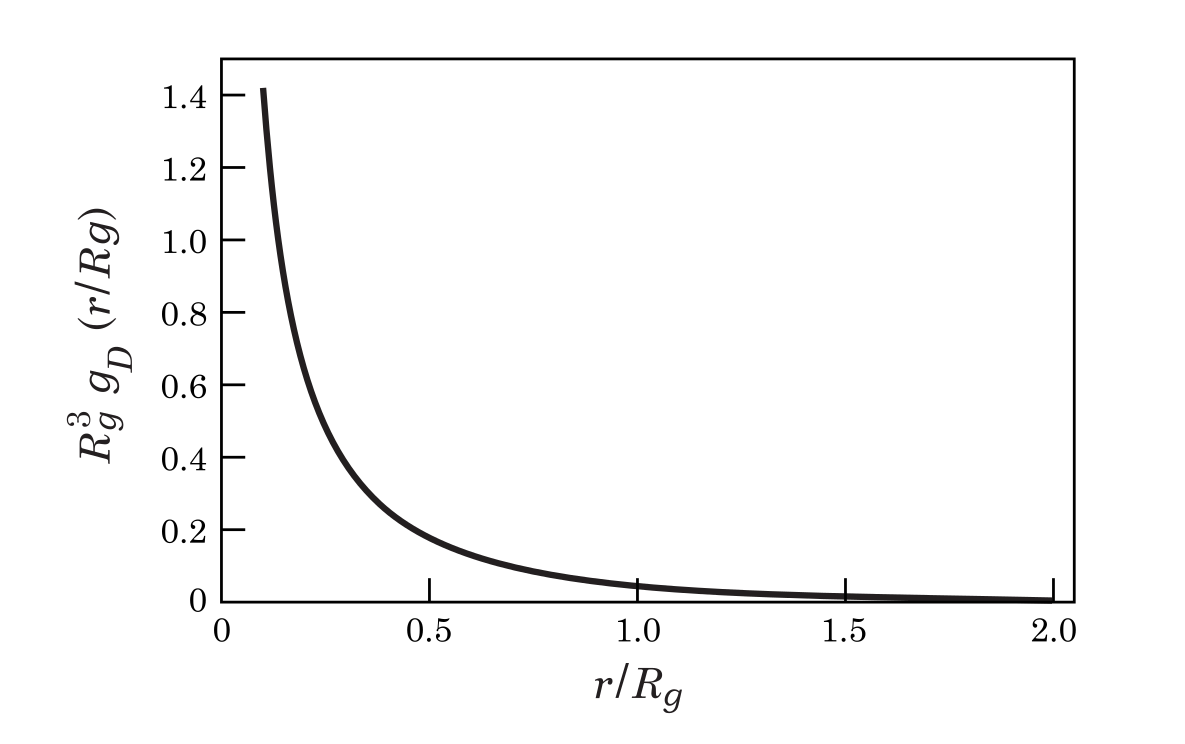
\includegraphics[scale=0.4]{./figures/FIG3-9.png}
	\caption{由(\ref{3.113})定义的Debye函数逆傅里叶变换,并以$\frac{r}{R_g}$为横坐标,以${R_g}^3 g_D(r)$为纵坐标.}
	\label{FIG3.9}
\end{figure}

形如(\ref{FIG3.9}),$\frac{r}{R_g} \ll 1$时,函数以$\frac{1}{r}$的速度代数衰减:
\begin{equation}
g_D(r) \sim \frac{3}{\pi b^2 N r}
\end{equation}
$r \sim R_g$时,函数单调的指数级的衰减为零:
$$g_D(r) \sim \frac{1}{r} e^{-\frac{\sqrt{3}r}{R_g}}$$

将弱非均匀性展开应用到其他聚合物体系(包括支链聚合物,共聚物)是非常直接的.

例如,在三臂星形均聚物的情况下,臂长相等,即$N_j = N$,
则
\begin{equation}
Q[w] = \frac{1}{V} \int [q(\mathbf{r},N;[w])]^3\,\mathrm{d} \mathbf{r}
\end{equation}
又由(\ref{3.116})和(\ref{3.119})可得
\begin{equation}
Q[w] \sim e^{-3w_0 N} [1+\frac{3 {\epsilon_a}^2 N^2}{2V^2} \sum_{\mathbf{k}} \hat{g_S}(k^2 {R_g}^2)\hat{\omega}(\mathbf{k})\hat{\omega}(-\mathbf{k})+\dots]
\end{equation}
其中${R_g}^2 = \frac{Nb^2}{6}$为星形中一臂的旋转半径,$g_S(x)$为类Debye函数
\begin{equation}
\hat{g_S}(x) = \hat{g_D}(x) + 2[\hat{h_D}(x)]^2
\end{equation}
其中
\begin{equation}
\hat{h_D}(x) = \frac{1}{x} [1-e^{-x}]
\end{equation}
从而密度算子和对相关函数分别为
\begin{equation}
\rho(\mathbf{r};[w]) \sim \rho_0[1-\epsilon_a N \int g_S(|\mathbf{r}-\mathbf{r}') \omega(\mathbf{r}')\,\mathrm{d} \mathbf{r}'+O({\epsilon_a}^2)]
\end{equation}

